% Curiosity Trainer Manual
% KOMA-Script book: Part I = development environment (VS Code + MPLAB),
% Part II = programming reference of the firmware drivers.
% Build with:  latexmk -pdf curiosity-trainer-manual.tex   (or pdflatex/lualatex, run twice)
\documentclass[
  11pt,
  letterpaper,
  oneside,
  DIV=13,               % text area size: higher = smaller margins
  parskip=half,          % space between paragraphs instead of indentation
  headings=normal,
  chapterprefix=false,
  toc=listof,
  numbers=noenddot,
]{scrbook}

\usepackage{iftex}
\ifPDFTeX
  \usepackage[T1]{fontenc}
  \usepackage[utf8]{inputenc}
  \usepackage{lmodern}
  \usepackage{textcomp}
\else
  \usepackage{fontspec}
\fi
\usepackage[english]{babel}
\usepackage{microtype}
\usepackage{amsmath}
\usepackage{graphicx}
\usepackage{xcolor}
\usepackage{array}
\usepackage{booktabs}
\usepackage{tabularx}
\usepackage{longtable}
\usepackage{enumitem}
\usepackage{listings}
\usepackage{tcolorbox}
\usepackage[automark,headsepline]{scrlayer-scrpage}
\usepackage[hidelinks]{hyperref}
\usepackage{bookmark}

% ---------- colors and page style ----------
\definecolor{accent}{HTML}{1F4E79}
\definecolor{codebg}{HTML}{F4F4F4}
\definecolor{codeframe}{HTML}{D0D0D0}
\addtokomafont{disposition}{\color{accent}}
\addtokomafont{minisec}{\color{accent}}
\setkomafont{pageheadfoot}{\normalfont\small\color{black!60}}
\pagestyle{scrheadings}
\clearpairofpagestyles
\ihead{\leftmark}
\ohead{\pagemark}
\setcounter{secnumdepth}{2}
\setcounter{tocdepth}{2}

% ---------- lists, tables ----------
\setlist{itemsep=0.2em, topsep=0.3em}
\renewcommand{\arraystretch}{1.25}
% two-column function tables and header tables converted from the reference
\newenvironment{functiontable}[1]
  {\par\smallskip\noindent\small\tabularx{\linewidth}{#1}}
  {\endtabularx\par\medskip}
\newenvironment{datatable}[1]
  {\par\smallskip\noindent\small\tabularx{\linewidth}{#1}}
  {\endtabularx\par\medskip}

% ---------- code ----------
\lstdefinestyle{c}{
  language=C,
  basicstyle=\ttfamily\small,
  keywordstyle=\color{accent}\bfseries,
  commentstyle=\color{black!55}\itshape,
  stringstyle=\color{green!40!black},
  backgroundcolor=\color{codebg},
  frame=single, rulecolor=\color{codeframe},
  framesep=4pt, xleftmargin=6pt, xrightmargin=6pt,
  breaklines=true, columns=fullflexible, keepspaces=true,
  showstringspaces=false, upquote=true, tabsize=4,
}
\lstdefinestyle{shell}{style=c, language={}, keywordstyle={}}
\lstset{style=c}

% ---------- note box ----------
\newtcolorbox{notebox}{colback=accent!6, colframe=accent, boxrule=0pt, leftrule=3pt,
  arc=0pt, left=8pt, right=8pt, top=4pt, bottom=4pt, before skip=8pt, after skip=10pt}

\hypersetup{
  pdftitle={Curiosity Trainer Manual},
  pdfsubject={Development environment and programming reference},
}

\begin{document}

% ---------- title page ----------
\begin{titlepage}
  \centering
  \vspace*{2cm}
  
\includegraphics[width=4cm]{figures/kettering-logo.png}\par
  \vspace{1.5cm}
  {\usekomafont{title}\color{accent}\Huge Curiosity Trainer Manual\par}
  \vspace{0.6cm}
  {\Large Development environment and programming reference\par}
  \vspace{0.4cm}
  {\large Curiosity Nano dsPIC33CK64MC105 training board\par}
  \vfill
  {\large Kettering University\par}
  \vspace{0.3cm}
  {\normalsize Osfield Gaga \& Jeremy Gooch\par}
  \vspace{0.3cm}
  {\normalsize\today\par}
\end{titlepage}

\frontmatter
\tableofcontents
\listoffigures

\mainmatter

\part{Development Environment}\label{part-environment}

\chapter{Overview}\label{ch-env-overview}

This part explains how to set up VS Code with the Microchip MPLAB extensions to build, program and debug the Curiosity Trainer firmware (dsPIC33CK64MC105 on a Curiosity Nano board). It follows the exact configuration used to develop the project, listed in chapter \ref{ch-env-config}, so that everyone works with the same versions. Part \ref{part-reference} then documents the firmware itself.

You will install, in this order:
\begin{enumerate}
\item VS Code.
\item The XC16 compiler, v2.10.
\item The MPLAB extensions for VS Code, which download the rest of the tools on first start.
\item On Linux only, the USB permissions for the board's debugger.
\item Optionally, MPLAB X IDE (command line programming), Python and MATLAB (microphone viewer).
\end{enumerate}
\begin{notebox}\textbf{Saved configuration:} the folder \texttt{docs/\allowbreak{}dev-\allowbreak{}environment} of the project keeps a copy of this configuration: the exact versions (\texttt{environment.\allowbreak{}json}), the list of extensions with install scripts, the project's VS Code settings and the Linux USB rule. Chapter \ref{ch-env-saved} explains how to use and refresh it.\end{notebox}

\chapter{Reference Configuration}\label{ch-env-config}

These are the versions installed on the development machine (captured on 2026-11-17). Newer versions usually work, but when something does not build or does not connect, these are the versions known to work.
\begin{longtable}{>{\raggedright\arraybackslash}p{0.22\linewidth}>{\raggedright\arraybackslash}p{0.30\linewidth}>{\raggedright\arraybackslash}p{0.40\linewidth}}
\toprule
\textbf{Component} & \textbf{Version} & \textbf{Notes} \\
\midrule
\endfirsthead
\toprule
\textbf{Component} & \textbf{Version} & \textbf{Notes} \\
\midrule
\endhead
\bottomrule
\endlastfoot
Operating system & Debian GNU/Linux 13 (trixie) & Kernel 6.12.113+deb13-amd64. The tools also exist for Windows and macOS \\
VS Code & 1.144.0 & Any recent version should work \\
MPLAB Extension Pack & 1.2.9 & Full list of extensions in chapter \ref{ch-env-ext} \\
XC16 compiler & v2.10 & Installed in \texttt{/\allowbreak{}opt/\allowbreak{}microchip/\allowbreak{}xc16/\allowbreak{}v2.\allowbreak{}10}. v2.00 is also installed but not used \\
Device pack (DFP) & dsPIC33CK-MC\_DFP 1.11.412 & Used by the VS Code project. The MPLAB X project files use 1.5.126 (also installed: 1.5.126, 1.6.238, 1.11.412) \\
Tool pack & nEDBG\_TP 1.20.1186 & Firmware support for the board's on-board debugger \\
MPLAB tools (downloaded by the extension) & make v4.4.1, ninja v1.13.2, hexmate v3.00, Java v21.0.13, backend 0.4.1065 & Installed automatically in \texttt{\textasciitilde{}/\allowbreak{}.\allowbreak{}mplab/\allowbreak{}app-\allowbreak{}finder/\allowbreak{}apps} \\
MPLAB X IDE (optional) & v6.05 & Command line programming (\texttt{ipecmd}) and the MPLAB X project in \texttt{nbproject/\allowbreak{}} \\
Board & Curiosity Nano dsPIC33CK64MC105 & On-board nEDBG debugger, listed as "PKOB nano" by the tools \\
Python (optional) & 3.13.5 & pyserial 3.5, numpy 2.2.4, matplotlib 3.10.1+dfsg1 (microphone viewer) \\
MATLAB (optional) & R2025a & With the MATLAB extension (microphone viewer) \\
\end{longtable}

\chapter{VS Code Extensions}\label{ch-env-ext}

The MPLAB Extension Pack installs all the Microchip extensions at once. The Microsoft C/C++ and CMake extensions are installed with it. The Python and MATLAB extensions are only needed for the microphone viewer scripts in \texttt{tools/\allowbreak{}}.
\begin{longtable}{>{\raggedright\arraybackslash}p{0.42\linewidth}>{\raggedright\arraybackslash}p{0.12\linewidth}>{\raggedright\arraybackslash}p{0.38\linewidth}}
\toprule
\textbf{Extension} & \textbf{Version} & \textbf{Role} \\
\midrule
\endfirsthead
\toprule
\textbf{Extension} & \textbf{Version} & \textbf{Role} \\
\midrule
\endhead
\bottomrule
\endlastfoot
\texttt{microchip.\allowbreak{}mplab-\allowbreak{}extension-\allowbreak{}pack} & 1.2.9 & Installs the whole MPLAB set below in one step \\
\texttt{microchip.\allowbreak{}mplab-\allowbreak{}ai-\allowbreak{}coding-\allowbreak{}assistant} & 1.2.4 & Microchip AI assistant (optional) \\
\texttt{microchip.\allowbreak{}mplab-\allowbreak{}clangd} & 2.1.0 & Code completion and navigation for XC16 code \\
\texttt{microchip.\allowbreak{}mplab-\allowbreak{}code-\allowbreak{}configurator} & 1.0.7 & MCC code generator (not used by this project) \\
\texttt{microchip.\allowbreak{}mplab-\allowbreak{}core-\allowbreak{}da} & 2.2.0 & Debugger and programmer (the mplab-core-da launch type) \\
\texttt{microchip.\allowbreak{}mplab-\allowbreak{}data-\allowbreak{}visualizer} & 0.1.5 & Serial terminal and plots for the debugger's COM port \\
\texttt{microchip.\allowbreak{}mplab-\allowbreak{}extensions-\allowbreak{}core} & 2.4.2 & Projects, build, the MPLAB view \\
\texttt{microchip.\allowbreak{}mplab-\allowbreak{}extensions-\allowbreak{}platforms} & 2.1.1 & Downloads and runs the MPLAB tools (backend, make, ninja, Java) \\
\texttt{microchip.\allowbreak{}mplab-\allowbreak{}kconfig} & 1.6.0 & Kconfig support (not used by this project) \\
\texttt{microchip.\allowbreak{}mplab-\allowbreak{}ui} & 2.2.3 & MPLAB user interface: project properties, packs, tools \\
\texttt{microchip.\allowbreak{}mplabx-\allowbreak{}importer} & 2.2.0 & Imports an MPLAB X project (.X folder) into VS Code \\
\texttt{microchip.\allowbreak{}runcmake} & 1.11.0 & Generates the CMake/ninja build of the project \\
\texttt{microchip.\allowbreak{}toolchains} & 1.11.3 & Finds the XC compilers (XC16 for this project) \\
\texttt{ms-\allowbreak{}vscode.\allowbreak{}cmake-\allowbreak{}tools} & 1.25.10 & CMake support, used by the MPLAB build \\
\texttt{ms-\allowbreak{}vscode.\allowbreak{}cpptools} & 1.35.6 & C/C++ language support \\
\texttt{ms-\allowbreak{}vscode.\allowbreak{}cpptools-\allowbreak{}extension-\allowbreak{}pack} & 1.5.1 & C/C++ extension pack \\
\texttt{ms-\allowbreak{}vscode.\allowbreak{}cpptools-\allowbreak{}themes} & 2.0.0 & C/C++ color themes \\
\texttt{ms-\allowbreak{}python.\allowbreak{}debugpy} & 2026.6.0 & Python debugger (optional) \\
\texttt{ms-\allowbreak{}python.\allowbreak{}python} & 2026.10.0 & Python, for tools/mic\_viewer.py (optional) \\
\texttt{ms-\allowbreak{}python.\allowbreak{}vscode-\allowbreak{}pylance} & 2026.4.1 & Python language server (optional) \\
\texttt{ms-\allowbreak{}python.\allowbreak{}vscode-\allowbreak{}python-\allowbreak{}envs} & 1.44.0 & Python environments (optional) \\
\texttt{mathworks.\allowbreak{}language-\allowbreak{}matlab} & 1.3.16 & MATLAB, for tools/mic\_viewer.m (optional) \\
\end{longtable}

\chapter{Installation}\label{ch-env-install}

\section{Install VS Code}

Download VS Code from code.visualstudio.com and install it (on Debian or Ubuntu, the .deb package). The \texttt{code} command must work in a terminal: the install scripts of chapter \ref{ch-env-saved} use it.

\section{Install the XC16 compiler}\label{sec-env-xc16}

The firmware is compiled with \textbf{MPLAB XC16 v2.10}. Download it from the Microchip website (MPLAB XC16 Compiler, downloads archive for older versions) and run the installer:
\begin{itemize}
\item \textbf{Linux:} make the installer executable and run it as root (the file name below is an example, use the name of the file you downloaded). It installs to \texttt{/\allowbreak{}opt/\allowbreak{}microchip/\allowbreak{}xc16/\allowbreak{}v2.\allowbreak{}10}.
\item \textbf{Windows:} run the installer, the default folder is \texttt{C:\textbackslash{}Program Files\textbackslash{}Microchip\textbackslash{}xc16\textbackslash{}v2.\allowbreak{}10}.
\item Choose the \textbf{free} license when asked: it is enough for this project (it compiles at -O0, the optimization level used by the project).
\item Keep the default install folder: the MPLAB extension looks for the compilers there.
\end{itemize}
\begin{lstlisting}[style=shell]
chmod +x xc16-v2.10-full-install-linux64-installer.run
sudo ./xc16-v2.10-full-install-linux64-installer.run
\end{lstlisting}

Check the installation in a terminal (Linux path shown):
\begin{lstlisting}[style=shell]
/opt/microchip/xc16/v2.10/bin/xc16-gcc --version
# elf-gcc (Microchip Technology) 4.5.1 (XC16, Microchip v2.10) ...
\end{lstlisting}

\section{Install the MPLAB extensions}\label{sec-env-ext}

Either install the extension pack from VS Code, or install the exact versions of chapter \ref{ch-env-ext} with the script.

\subsection{Option A: from VS Code (latest versions)}
\begin{enumerate}
\item Open the Extensions view (Ctrl+Shift+X).
\item Search for \textbf{MPLAB Extension Pack} (publisher: Microchip Technology) and click Install.
\item Restart VS Code when asked.
\end{enumerate}

\subsection{Option B: exact versions with the script}

From the project folder, run the script for your system. Add \texttt{-{}-\allowbreak{}latest} (Linux) or \texttt{-\allowbreak{}Latest} (Windows) to install the same extensions in their newest versions.
\begin{lstlisting}[style=shell]
# Linux / macOS
./docs/dev-environment/install-vscode-extensions.sh

# Windows (PowerShell)
.\docs\dev-environment\install-vscode-extensions.ps1
\end{lstlisting}

\subsection{First start}

The first time VS Code starts with the extensions, they download their own tools: the MPLAB backend, make, ninja, hexmate and a Java runtime (Linux: \texttt{\textasciitilde{}/\allowbreak{}.\allowbreak{}mplab/\allowbreak{}app-\allowbreak{}finder/\allowbreak{}apps}). This needs an internet connection and can take a few minutes: wait for the downloads shown in the status bar and the notifications to finish before opening the project.

\section{Linux only: USB access to the board}\label{sec-env-usb}

Without these permissions, the board is not found by the tools and the serial port cannot be opened. Installing MPLAB X IDE also installs the udev rule, otherwise use the copy saved in the project:
\begin{lstlisting}[style=shell]
sudo cp docs/dev-environment/linux/z010_mchp_tools.rules /etc/udev/rules.d/
sudo udevadm control --reload-rules && sudo udevadm trigger
sudo usermod -aG dialout $USER     # access to /dev/ttyACM* (serial port)
\end{lstlisting}

Log out and back in (or reboot) for the group change to apply, then unplug and replug the board.

\section{Optional tools}
\begin{itemize}
\item \textbf{MPLAB X IDE v6.05:} used for command line programming (\texttt{ipecmd}, \texttt{mdb}) and to open the MPLAB X project files in \texttt{nbproject/\allowbreak{}}. Not needed to work in VS Code.
\item \textbf{Python 3} with the packages of the microphone viewer: \texttt{pip install pyserial numpy matplotlib}.
\item \textbf{MATLAB} (R2025a used, \texttt{serialport} is part of base MATLAB) for \texttt{tools/\allowbreak{}mic\_\allowbreak{}viewer.\allowbreak{}m}.
\end{itemize}

\chapter{Opening the Project}\label{ch-env-open}
\begin{enumerate}
\item Plug in the Curiosity Nano board with a USB-C cable.
\item In VS Code, use File > Open Folder and select the \texttt{CuriosityTrainer.\allowbreak{}X} folder.
\item The MPLAB extension reads the project from \texttt{.\allowbreak{}vscode/\allowbreak{}CuriosityTrainer.\allowbreak{}mplab.\allowbreak{}json} and shows the project \textbf{CuriosityTrainer}, configuration \textbf{default}, in the MPLAB view.
\item If the extension asks to download the device pack (dsPIC33CK-MC\_DFP) or the tool pack (nEDBG\_TP), accept: packs are stored in \texttt{\textasciitilde{}/\allowbreak{}.\allowbreak{}mchp\_\allowbreak{}packs}.
\item When asked for the tool, select the board's debugger, listed as \textbf{PKOB nano} with its serial number. The choice is saved in \texttt{.\allowbreak{}vscode/\allowbreak{}CuriosityTrainer.\allowbreak{}mplab-\allowbreak{}local.\allowbreak{}json}, which is specific to each computer and board.
\end{enumerate}

If the \texttt{.\allowbreak{}vscode} folder is missing (for example in a fresh copy of the repository), either copy the files of \texttt{docs/\allowbreak{}dev-\allowbreak{}environment/\allowbreak{}vscode} into \texttt{.\allowbreak{}vscode} (chapter \ref{ch-env-saved}), or import the MPLAB X project: open the Command Palette (Ctrl+Shift+P), type \textbf{Import}, choose the MPLAB X project import command and select the \texttt{CuriosityTrainer.\allowbreak{}X} folder.

\section{Project settings}

The project configuration (in the MPLAB project properties, or \texttt{.\allowbreak{}vscode/\allowbreak{}CuriosityTrainer.\allowbreak{}mplab.\allowbreak{}json}) must match these values:
\begin{longtable}{>{\raggedright\arraybackslash}p{0.25\linewidth}>{\raggedright\arraybackslash}p{0.67\linewidth}}
\toprule
\textbf{Setting} & \textbf{Value} \\
\midrule
\endfirsthead
\toprule
\textbf{Setting} & \textbf{Value} \\
\midrule
\endhead
\bottomrule
\endlastfoot
Device & dsPIC33CK64MC105 \\
Toolchain & XC16 v2.10 (property group \texttt{default-\allowbreak{}XC16}, provider \texttt{microchip.\allowbreak{}toolchains:xc16@2.\allowbreak{}10}) \\
Device pack & dsPIC33CK-MC\_DFP 1.11.412 \\
Tool & PKOB nano (the board's nEDBG debugger) \\
Optimization & -O0, symbols enabled, all warnings \\
Memory models & Small code, small data \\
Source files & All \texttt{*.\allowbreak{}c}, \texttt{*.\allowbreak{}h} and \texttt{*.\allowbreak{}s} files of the project folder (new files are picked up automatically) \\
\end{longtable}

\chapter{Build, Program and Debug}\label{ch-env-build}
\begin{itemize}
\item \textbf{Build:} run the build task \textbf{CuriosityTrainer: default - Build} (Terminal > Run Build Task, or the build button of the MPLAB view). The output is \texttt{out/\allowbreak{}CuriosityTrainer/\allowbreak{}default.\allowbreak{}elf}.
\item \textbf{Program the board:} in the Run and Debug view (Ctrl+Shift+D), start \textbf{Program CuriosityTrainer: default - Production}. It builds the production image and programs it without debugging.
\item \textbf{Debug:} start \textbf{Launch CuriosityTrainer: default}. It builds, programs and stops at the start of \texttt{main()}; use the usual VS Code debug controls (breakpoints, step, variables).
\item \textbf{Serial port:} the board's debugger also provides a virtual COM port (\texttt{/\allowbreak{}dev/\allowbreak{}ttyACM0} on Linux, a COM port on Windows). The examples use 9600 baud, the microphone example 115200 baud. Use the MPLAB Data Visualizer extension, any serial terminal or the viewers in \texttt{tools/\allowbreak{}}. Only one program can open the port at a time.
\end{itemize}
\begin{notebox}\textbf{Tip:} the first build after opening the project takes longer: the extension generates the CMake build files in \texttt{cmake/\allowbreak{}} and \texttt{\_\allowbreak{}build/\allowbreak{}}.\end{notebox}

\chapter{Saved Configuration}\label{ch-env-saved}

The folder \texttt{docs/\allowbreak{}dev-\allowbreak{}environment} keeps this configuration with the project, so it is not lost when a computer is replaced:
\begin{longtable}{>{\raggedright\arraybackslash}p{0.36\linewidth}>{\raggedright\arraybackslash}p{0.56\linewidth}}
\toprule
\textbf{File} & \textbf{Content} \\
\midrule
\endfirsthead
\toprule
\textbf{File} & \textbf{Content} \\
\midrule
\endhead
\bottomrule
\endlastfoot
\texttt{environment.\allowbreak{}json} & Versions of the OS, VS Code, XC16, MPLAB X, packs, MPLAB tools, Python and MATLAB \\
\texttt{vscode-\allowbreak{}extensions.\allowbreak{}txt} & The VS Code extensions with their exact versions \\
\texttt{install-\allowbreak{}vscode-\allowbreak{}extensions.\allowbreak{}sh} / \texttt{.\allowbreak{}ps1} & Install the extensions of the list (Linux or macOS / Windows) \\
\texttt{capture\_\allowbreak{}environment.\allowbreak{}sh} & Regenerates \texttt{environment.\allowbreak{}json} and \texttt{vscode-\allowbreak{}extensions.\allowbreak{}txt} from the current computer \\
\texttt{vscode/\allowbreak{}} & The project's \texttt{.\allowbreak{}vscode} files: MPLAB project, launch configurations, settings \\
\texttt{linux/\allowbreak{}z010\_\allowbreak{}mchp\_\allowbreak{}tools.\allowbreak{}rules} & Microchip udev rule for USB access (Linux) \\
\end{longtable}

\section{Restoring the VS Code configuration}

Copy the files of \texttt{docs/\allowbreak{}dev-\allowbreak{}environment/\allowbreak{}vscode} into the project's \texttt{.\allowbreak{}vscode} folder. \texttt{CuriosityTrainer.\allowbreak{}mplab-\allowbreak{}local.\allowbreak{}example.\allowbreak{}json} only shows the format of the per-computer file: the extension creates the real \texttt{CuriosityTrainer.\allowbreak{}mplab-\allowbreak{}local.\allowbreak{}json} when you select the board.

Differences with the original \texttt{.\allowbreak{}vscode} files, made so the copy works on any computer:
\begin{itemize}
\item \texttt{settings.\allowbreak{}json}: \texttt{cmake.\allowbreak{}sourceDirectory} used an absolute path of the development computer, it now uses \texttt{\$\{workspaceFolder\}}.
\item \texttt{launch.\allowbreak{}json}: only the configurations of the \textbf{default} project configuration are kept. The original also had entries for a \textbf{curiosity} configuration that does not exist in the project.
\end{itemize}

\section{Refreshing the snapshot}

After updating VS Code, the extensions, the compiler or the packs, run the capture script on Linux and commit the updated files:
\begin{lstlisting}[style=shell]
./docs/dev-environment/capture_environment.sh
\end{lstlisting}

\chapter{Troubleshooting the Environment}\label{ch-env-trouble}

Problems with the firmware itself are covered in chapter \ref{ch-common-problems}.

\section{The board is not found, or the serial port cannot be opened (Linux)}

Check the udev rule and the dialout group (section \ref{sec-env-usb}), then unplug and replug the board. \texttt{lsusb} should list the debugger as \texttt{03eb:2175 Atmel Corp.\allowbreak{} nEDBG CMSIS-\allowbreak{}DAP}.

\section{"Unrecoverable error while communicating with the PKOB nano", USB errors -109 or -150}

The debugger lost its USB connection: unplug and replug the board, then start again. Very high UART baud rates (1000000 and above) on the virtual COM port can crash the debugger, and it drops bytes from 500000 baud: keep the UART at 250000 baud or below.

\section{The compiler is not found or not offered as a toolchain}

Check that XC16 v2.10 is installed in its default folder (section \ref{sec-env-xc16}), then restart VS Code so the toolchains extension finds it again.

\section{The device pack version does not match}

The VS Code project uses dsPIC33CK-MC\_DFP 1.11.412, while the MPLAB X project files (\texttt{nbproject/\allowbreak{}}) were made with 1.5.126. Both work: install the version the tool asks for, the packs can be installed side by side.

\section{The tools are still downloading, or the MPLAB view stays empty}

On the first start, wait for the MPLAB extensions to finish downloading their tools (section \ref{sec-env-ext}), then reload the window (Ctrl+Shift+P, Developer: Reload Window).

\part{Programming Reference}\label{part-reference}

\chapter{Introduction}

This document serves as a comprehensive technical guide for working with the Curiosity Nano training board and the Microchip \textbf{XC16 compiler}. It provides the necessary documentation for the hardware-specific libraries designed to streamline the development of embedded applications.

\section{Purpose and Configuration}

The board boots from the Internal Fast RC (\textbf{FRC}) oscillator (8 MHz), then main() switches to FRC + PLL: the system clock Fosc is \textbf{32 MHz} and the instruction/peripheral clock Fcy = Fp is \textbf{16 MHz}.

A central component of this firmware framework is \textbf{Timer 1}, which is initialized to trigger an interrupt every \textbf{millisecond}. This interrupt provides a continuous background counter (msCount) and a periodic trigger flag (tFlag) essential for timing-sensitive operations, such as refreshing the seven-segment display.

\section{Document Structure}

To ensure proper hardware initialization, users should always include config.h in their main.c file. The reference is organized into two primary categories:
\begin{itemize}
\item \textbf{Low-Level Modules:} Detailed documentation for fundamental peripherals including the \textbf{ADC}, \textbf{PWM}, \textbf{SCCP}, \textbf{UART} and the \textbf{I2C} bus.
\item \textbf{High-Level Modules:} Usage guides for integrated components such as the \textbf{Keypad}, \textbf{4-digit 7-Segment Display}, \textbf{Switches}, \textbf{LEDs}, \textbf{OLED Display}, \textbf{IO Expander}, and various sensors like the \textbf{Photoresistor}, \textbf{Ultrasonic Distance Sensor}, \textbf{Accelerometer} and \textbf{Microphone}.
\end{itemize}

Each section includes file requirements, function definitions, and "Example Usage" snippets to help you quickly integrate these features into your projects.

\chapter{Useful references}
\begin{itemize}
\item Microchip XC16 reference: useful for interrupt definitions
\end{itemize}

\chapter{Configuration}

The config.c file contains the main initialization and configuration of the board. Setting up these registers was done using code generated by MCC Configurator, as recommended by Microchip. Without these configurations, a couple of pins are overridden by the debugger, thus cannot be used as GPIOs. It is neither recommended nor necessary to change the configuration for most, if not all of the use cases of this training board. However, if required, the Oscillator Source can be changed by setting \textbf{\#pragma config FNOSC} to the desired source. Doing so, or changing the PLL setup at the start of main(), would require updating FCY in config.h, Timer 1's period, the SCCP prescaler, the PWM clock divider and the neopixel bit timing. By default, the FRC (8 MHz) feeds the PLL, giving a system clock Fosc of 32 MHz and Fcy = Fp = 16 MHz.

At the heart of this set of libraries is an interrupt triggered by Timer 1. Due to the lack of a Core Timer (available on other microcontroller families), \textbf{\_T1Interrupt }is set to run in the background to provide a continuous millisecond counter and a periodic flag whose period can be adjusted as required. The millisecond counter \textbf{msCount }and the periodic flag \textbf{tFlag} are accessible wherever ``config.h'' is included.

In the config.h header file, the period of the periodic flag previously mentioned is set by defining the macro \textbf{T1\_TIME\_MS} in \textbf{milliseconds}. The default value is set to 1000 milliseconds, or 1 second. The flag itself can be used by accessing its variable \textbf{tFlag}. It is important to set tFlag to 0 every time it is called if it is desired to have it run as a periodic trigger. Not setting back to 0 essentially stops the flag from triggering.

The period at which Timer1's interrupt triggers is set using \textbf{T1\_PERIOD}, also in the config.h header file. By default, Timer1 is set to use a 1:8 prescaler. Since $F_{\mathrm{PB}}$ (the peripheral bus clock) is half of the system clock Fosc, we have
\[ F_{\mathrm{PB}} = \frac{F_{\mathrm{osc}}}{2} \]
\[ F_{\mathrm{PB}} = \frac{32\,\mathrm{MHz}}{2} = 16\,\mathrm{MHz} \]

Since Timer 1 is set with a 1:8 prescaler, the frequency at which it increments its internal counter TMR1 is defined by
\[ F_{\mathrm{T1}} = \frac{16\,\mathrm{MHz}}{8} = 2\,\mathrm{MHz} = 2\,000\,000\,\mathrm{Hz} \]

To obtain a timer that increments its counter once every millisecond, we need to divide $F_{\mathrm{T1}}$ by 1000, which equals 2000. The timer counts from 0 up to and including its period, so \textbf{T1\_PERIOD }is set to 2000 $-$ 1 = 1999.

\textbf{FCY} (16 MHz) is also defined in config.h. It is used by \_\_delay\_ms() and \_\_delay\_us() from libpic30.h and by the UART baud rate calculation, so config.h must always be included before libpic30.h.
\minisec{Files}

config.c and config.h
\minisec{Functions}
\begin{functiontable}{>{\raggedright\arraybackslash}p{0.36\linewidth}>{\raggedright\arraybackslash}X}
\toprule
\textbf{init\_T1()} & Initializes Timer1 to trigger and interrupt every millisecond \\
\bottomrule
\end{functiontable}

\textbf{Note:} The seven segment relies on Timer 1 to set its refresh rate, changing the period of Timer 1 will affect how digits are displayed.
\minisec{Usage}

Include config.h in the main.c file to ensure the board is configured properly.
\begin{lstlisting}
#include "config.h"
\end{lstlisting}

\chapter{Modules \& Peripherals}

\section{Low-level}

\subsection{ADC}

The Analog-toDigital module is initialized using the ADC\_Init function.The function sets up the shared ADC Core. By default, the clock is selected as the peripheral clock with no clock divider.

The ADC module itself needs to be enabled by setting ADCON1Lbits.ADON to 1. This enables the entire ADC peripherals (ADC Core, ADC1, etc.). ADCON5Lbits.SHRPWR provides power to the ADC Core, and finally ADCON3Hbits.SHREN enables the ADC core specifically. Enabling the ADC core should be done when it is ready, thus waiting for ADCON5Lbits.SHRRDY to be set to 1.

Setting up the ADC does not automatically assign the channel to use, this initialization is meant to be wrapped in a function that explicitly specifies the channel to be used for a specific application or component.
\minisec{Files}

adc.c and adc.h
\minisec{Functions}
\begin{functiontable}{>{\raggedright\arraybackslash}p{0.36\linewidth}>{\raggedright\arraybackslash}X}
\toprule
\textbf{ADC\_Init ()} & Initialize the ADC Core module \\
\textbf{ADC\_Set\_AN9()} & Assign AN9 to the ADC Core \\
\textbf{ADC\_Core\_Read()} & Samples and converts the analog voltage on AN9 \\
\bottomrule
\end{functiontable}

\textbf{Note:} ADC\_Set\_AN9() must always be called before ADC\_Core\_Read() else, no channel will be linked to the ADC Core module. This was done intentionally to allow the programmer to assign a different channel if required.
\minisec{Example usage}

Setting up the Potentiometer to use the AN9 channel, then converting the voltage from an analog value to its digital equivalent.
\begin{lstlisting}
#include "xc.h"
#include "config.h"
#include "adc.h"

void POT_Init(void) {
    // ... perform initialization of Pins
    ADC_Init();
}

int read_pot(float min, float max) {
    ADC_Set_AN9(); // set up the potentiometer to use AN9
    output = ADC_Core_Read(); // sample and convert voltage
}
\end{lstlisting}

\subsection{PWM}

The Curiosity Nano has 4 PWM modules. Only PWM4L is used on the training board. Due to the limited availability of the IO pins, PWM4L which was originally on pin RD1 has been remapped to pin RB7. PWM4 counts at Fosc / 16 = 2 MHz (master clock divided by the PCLKCON 1:16 divider), defined as FP in pwm.h. The period register value for a frequency f is therefore FP / f $-$ 1, and the 16-bit period register covers frequencies down to about 31 Hz.
\minisec{Files}

pwm.c and pwm.h
\minisec{Functions}
\begin{functiontable}{>{\raggedright\arraybackslash}p{0.36\linewidth}>{\raggedright\arraybackslash}X}
\toprule
\textbf{void PWM1\_Initialize(void)}\newline \textbf{void PWM2\_Initialize(void)}\newline \textbf{void PWM3\_Initialize(void)}\newline \textbf{void PWM4\_Initialize(void)} & Initialize the corresponding PWM module \\
\textbf{int freq\_to\_pgxper(int freq) (buzzer.c)} & Returns the corresponding PGxPER value for the desired frequency in Hz \\
\textbf{void PWM4\_Disable(void)} & Turns PWM4 off and releases RB7 (removes the PPS mapping and sets the pin as an input) \\
\bottomrule
\end{functiontable}
\minisec{Example usage}

Setting up PWM4, then changing it to a 1 kHz signal with a 50\% duty cycle
\begin{lstlisting}
#include "xc.h"
#include "config.h"
#include "pwm.h"

void main() {
    PWM4_Initialize();         // 130.8 Hz, 50% duty cycle on RB7

    PG4PER = (FP / 1000) - 1;  // 1 kHz
    PG4DC = PG4PER / 2;        // 50% duty cycle
    PG4STATbits.UPDREQ = 1;    // apply the new period and duty cycle

    while (1) {
    }
}
\end{lstlisting}

\subsection{SCCP}

The Single Capture/Compare/PWM module can either be used as a general purpose timer, input capture and output compare. On the training board, it is only initialized as an input capture module. This can be modified by the user if need be.

By default, the input compare is only used to interface the ultrasonic distance sensor. The module is initialized and  \emph{RPINR3bits.ICM1R } is set to the value corresponding to the ultrasonic sensor. The capture timer runs at Fcy / 16 = 1 MHz, so one tick is 1 \textmu{}s. SCCP\_Init() unlocks the Peripheral Pin Select (PPS) registers before writing RPINR3 and locks them again afterwards.
\minisec{Files}

sccp.c and sccp.h
\minisec{Functions}
\begin{functiontable}{>{\raggedright\arraybackslash}p{0.36\linewidth}>{\raggedright\arraybackslash}X}
\toprule
\textbf{void SCCP\_Init(void)} & Initialize the SCCP module and sets it in Input capture mode \\
\bottomrule
\end{functiontable}
\minisec{Example usage}

Setting up the SCCP module
\begin{lstlisting}
#include "xc.h"
#include "config.h"
#include "sccp.h"

void main() {
     SCCP_Init();

     while (1) {
       
     }

}
\end{lstlisting}

\subsection{UART}

UART communication can be achieved through the USB interface of the Curiosity Nano board. UART1 is routed through Peripheral Pin Select (PPS) to the debugger's virtual COM port: U1TX on RC10 (RP58) and U1RX on RC11 (RP59). UartInit() performs this mapping, so no hardware configuration is required. The default settings are 9600 baud, 8 data bits, no parity and 1 stop bit (9600 8N1). The baud rate is set by UART\_BAUD in uart.h and computed from FCY with the fine (BRGH = 1) divider: 9600 gives 9592 baud and 115200 gives 114286 baud. UartInitBaud() initializes the UART at any other rate.

The user can however initialize and use the other pins associated with a specific UART module. An external header is provided on the training board for UART communication to other components via a direct connection.

\textbf{Note:} some drivers lock the PPS registers (for example PWM4\_Disable()), and writes to RPORx / RPINRx made while PPS is locked are silently ignored. Any code that remaps pins must unlock PPS first with \_\_builtin\_write\_RPCON(0x0000) and lock it again with \_\_builtin\_write\_RPCON(0x0800). UartInit() and SCCP\_Init() already do this.
\minisec{Pins}
\begin{datatable}{>{\raggedright\arraybackslash}p{0.16\linewidth}>{\raggedright\arraybackslash}X>{\raggedright\arraybackslash}p{0.2\linewidth}}
\toprule
\textbf{Pin} & \textbf{Device} & \textbf{Direction} \\
\midrule
RC10 & U1TX (to debugger CDC RX) & OUT \\
RC11 & U1RX (from debugger CDC TX) & IN \\
\bottomrule
\end{datatable}
\minisec{Files}

uart.c and uart.h
\minisec{Functions}
\begin{functiontable}{>{\raggedright\arraybackslash}p{0.36\linewidth}>{\raggedright\arraybackslash}X}
\toprule
\textbf{void UartInit(void)} & Initialize the UART 1 module \\
\textbf{void UartSendByte(char data)} & Send a byte of data \\
\textbf{void UartSendString(char *pData)} & Send a string over UART \\
\textbf{void UartInitBaud(uint32\_t baud)} & Initialize the UART 1 module at any baud rate, for example 115200 or 250000 for fast data \\
\textbf{void UartSendBuffer(const uint8\_t *pData, uint16\_t len)} & Send raw bytes, zeros included (UartSendString() stops at the first 0) \\
\textbf{uint8\_t UartDataAvailable(void)} & Returns 1 if a received byte is waiting to be read. Also clears a receive overrun, which would otherwise stop the receiver \\
\textbf{char UartReadByte(void)} & Waits until a byte is received and returns it \\
\bottomrule
\end{functiontable}
\minisec{Example usage}

Setting up the UART, sending a welcome message, then echoing back every byte received
\begin{lstlisting}
#include "xc.h"
#include "config.h"
#include "uart.h"

void main() {
    UartInit();
    __delay_ms(100);
    UartSendString("\r\nWelcome!\r\n");

    while (1) {
        if (UartDataAvailable()) {
            char c = UartReadByte();
            UartSendByte(c); // echo the byte back
        }
    }
}
\end{lstlisting}

\subsection{I2C (software master)}

The OLED display, the IO expander and the accelerometer share one I2C bus on RC8 (SDA) and RC9 (SCL). The bus is driven in software by Microchip's dsPIC33C I2C software library (i2c\_master.c): it switches the two pins directly instead of using the I2C peripheral. Both pins are open-drain outputs (ODCC8 and ODCC9 = 1): a device pulls a line low, and the pull-up resistors of the bus bring it back high.

The bus speed is set by I2C\_CLOCK\_DELAY in i2c\_master.h (20 by default), the length of the delays between the edges of SCL. Measured on the board, the SCL period is 132 instruction cycles (8.25 \textmu{}s), a clock of about 121 kHz, well within the 400 kHz limit of the OLED controller and of the IO expander. A byte (8 bits and the acknowledge) takes about 76 \textmu{}s. Clock stretching is supported: the master waits while a device holds SCL low.

A transaction is built from the functions below: a start condition, the 7-bit device address shifted left with the read/write bit (0 = write, 1 = read), the data bytes, then a stop condition. To read a register, write the register number, then send a repeated start (I2CM\_Start() again, without a stop) followed by the address with the read bit. The addresses on the bus are 0x3C (OLED), 0x20 (IO expander) and 0x1D (accelerometer).

\textbf{Note: }I2CM\_Init() only sets up the two pins, so every driver of the bus calls it (init\_oled(), init\_IO\_expander() and init\_accelerometer()). The drivers do not check the values returned by I2CM\_Start(), I2CM\_Stop() and I2CM\_Write() (bus collision, no acknowledge): use the example below to check that a device answers.
\minisec{Pins}
\begin{datatable}{>{\raggedright\arraybackslash}p{0.16\linewidth}>{\raggedright\arraybackslash}X>{\raggedright\arraybackslash}p{0.2\linewidth}}
\toprule
\textbf{Pin} & \textbf{Device} & \textbf{Direction} \\
\midrule
RC8 & I2C SDA (OLED, IO expander, accelerometer) & IN/OUT, open drain \\
RC9 & I2C SCL (OLED, IO expander, accelerometer) & OUT, open drain \\
\bottomrule
\end{datatable}
\minisec{Files}

i2c\_master.c and i2c\_master.h (Microchip dsPIC33C I2C software library)
\minisec{Functions}
\begin{functiontable}{>{\raggedright\arraybackslash}p{0.36\linewidth}>{\raggedright\arraybackslash}X}
\toprule
\textbf{void I2CM\_Init()} & Sets SDA and SCL as open-drain outputs, both released high \\
\textbf{short I2CM\_Start()} & Generates a start condition, or a repeated start inside a transaction. Returns a non-zero value if the bus is busy (bus collision) \\
\textbf{short I2CM\_Stop()} & Generates a stop condition. Returns a non-zero value on a bus collision \\
\textbf{short I2CM\_Write(unsigned char data)} & Sends a byte and returns the acknowledge of the device: 0 = ACK, 1 = NACK (no device answered) \\
\textbf{unsigned char I2CM\_Read(short ack)} & Reads a byte. ack = 0 acknowledges it (more bytes follow), ack = 1 sends a NACK (last byte) \\
\bottomrule
\end{functiontable}
\minisec{Example usage}

Checking that a device answers, then reading one of its registers (here the input port of the IO expander)
\begin{lstlisting}
#include "xc.h"
#include "i2c_master.h"

uint8_t device_present(uint8_t addr) {
    short nack;
    I2CM_Start();
    nack = I2CM_Write(addr << 1);    // address + write bit
    I2CM_Stop();
    return !nack;                    // 1 if a device acknowledged
}

uint8_t read_register(uint8_t addr, uint8_t reg) {
    uint8_t value;
    I2CM_Start();
    I2CM_Write(addr << 1);           // address + write bit
    I2CM_Write(reg);                 // register to read
    I2CM_Start();                    // repeated start
    I2CM_Write((addr << 1) | 0x01);  // address + read bit
    value = I2CM_Read(1);            // last byte: NACK
    I2CM_Stop();
    return value;
}

void main() {
    I2CM_Init();
    if (device_present(0x20)) {
        uint8_t inputs = read_register(0x20, 0x00);
    }
}
\end{lstlisting}

\section{High-level}

\subsection{Keypad}

The keypad is 3 by 4 keys, for a total of 12 keys. It is not debounced by default, it is the responsibility of the programmer to debounce the keys to prevent repeated inputs.

The keyboard's row pins (ROW1 to ROW4)  are shared with the slide switches (SW1 to SW4, respectively).

\textbf{Keypad and switches SW1 to SW4: }the keypad and switches SW1 to SW4 cannot be used at the same time. While the keypad is in use, every switch that is ON ties its row to the other rows that are ON, so those rows cannot be told apart and readKey() returns the wrong key, or a key that is not pressed.

\textbf{Work around: }turn SW1 to SW4 OFF while using the keypad, and call keypad\_check\_rows() before readKey(). When it returns a non-zero value, ignore the keypad and ask the user to turn the switches off. Example 1 does this: it shows ``Keypad blocked!'' on the OLED and flashes ``-{}-{}-{}-'' on the 7 segment display until the switches are off (the OLED message refers to the switches as SW0 to SW3).
\minisec{Pins}
\begin{datatable}{>{\raggedright\arraybackslash}p{0.16\linewidth}>{\raggedright\arraybackslash}X>{\raggedright\arraybackslash}p{0.2\linewidth}}
\toprule
\textbf{Pin} & \textbf{Device} & \textbf{Direction} \\
\midrule
RC0 & Keypad COL2 & OUT \\
RC1 & Keypad COL1 & OUT \\
RC2 & Keypad ROW4 & IN \\
RC3 & Keypad ROW3 & IN \\
RC4 & Keypad ROW2 & IN \\
RC5 & Keypad ROW1 & IN \\
RA4 & Keypad COL3 & OUT \\
\bottomrule
\end{datatable}
\minisec{Files}

keypad.c and keypad.h
\minisec{Functions}
\begin{functiontable}{>{\raggedright\arraybackslash}p{0.36\linewidth}>{\raggedright\arraybackslash}X}
\toprule
\textbf{init\_keypad()} & Initialize the keypad pins \\
\textbf{readKey(uint8\_t outputMode)} & Reads the key and either returns a raw character or its decimal equivalent. \textbf{outputMode }is used to choose between decimal and char. It can be set to either \textbf{KEYPAD\_OUTPUT\_DECIMAL }or \textbf{KEYPAD\_OUTPUT\_CHAR}, both macros defined in keypad.h.\newline Example: \textbf{readKey(KEYPAD\_OUTPUT\_DECIMAL ) }and pressing `A' would return 15. \\
\textbf{uint8\_t keypad\_check\_rows(void)} & Checks whether switches SW1 to SW4 interfere with the keypad rows. Returns a bitmask of the affected rows (bit 0 = ROW1), 0 if the keypad can be used \\
\bottomrule
\end{functiontable}
\minisec{Example usage}

Initializing the keypad, checking the switches, then reading the key pressed
\begin{lstlisting}
#include "xc.h"
#include "config.h"
#include "keypad.h"

void main() {
    init_keypad();
    unsigned char key_in;

    while (1) {
        if (keypad_check_rows()) {
            // SW1 to SW4 are ON: the keys can't be read, ask to turn them off
            continue;
        }

        key_in = readKey(KEYPAD_OUTPUT_CHAR);
        // do something with the key pressed
    }
}
\end{lstlisting}

\subsection{7 Segment Display}

The board features a 4 digit 7 segment display. The display is refreshed every millisecond using the running Timer 1 interrupt. The refreshing of the display can be enabled or disabled with the \emph{seven\_seg\_enable }global variable/flag. If not in use, the flag should be set to 0.
\minisec{Pins}
\begin{datatable}{>{\raggedright\arraybackslash}p{0.16\linewidth}>{\raggedright\arraybackslash}X>{\raggedright\arraybackslash}p{0.2\linewidth}}
\toprule
\textbf{Pin} & \textbf{Device} & \textbf{Direction} \\
\midrule
RC6 & 7 seg - 11 (A) & OUT \\
RC7 & 7 seg - 7 (B) & OUT \\
RC12 & 7 seg - 4 (C) & OUT \\
RC13 & 7 seg - 2 (D) & OUT \\
RD10 & 7 seg -  1 (E) & OUT \\
RA0 & 7 seg - 10 (F) & OUT \\
RB2 & 7 seg - 5 (G) & OUT \\
RB9 & 7 seg - 12 (DIG1) & OUT \\
RA3 & 7 seg - 3 (DP) & OUT \\
RB10 & 7 seg - 9 (DIG2) & OUT \\
RD8 & 7 seg - 8 (DIG3) & OUT \\
RD1 & 7 seg - 6 (DIG4) & OUT \\
RA1 & 7 seg - Column & OUT \\
\bottomrule
\end{datatable}
\minisec{Files}

seven\_segment.c and seven\_segment.h
\minisec{Functions}
\begin{functiontable}{>{\raggedright\arraybackslash}p{0.36\linewidth}>{\raggedright\arraybackslash}X}
\toprule
\textbf{init\_seven\_seg()} & Initialize the seven segment display pins \\
\textbf{print\_seven\_seg(uint8\_t d0, uint8\_t d1, uint8\_t d2, uint8\_t d3)} & Displays the values of d0 to d3. DIG4 corresponds to d0, DIG3 to d1, DIG2 to d2 and DIG1 to d3 \\
\textbf{print\_decimal\_point(uint8\_t dp0, uint8\_t dp1, uint8\_t dp2, uint8\_t dp3)} & Controls the decimal points corresponding to each digit of the seven segment display. Setting each a value of 1 turns on the decimal point, and setting it to zero turns ot off \\
\textbf{refresh\_seven\_seg();} & Refreshed the seven segment display by cycling through each digit individually. This is called in the Timer 1 interrupt \\
\textbf{seven\_seg\_display\_off()} & Turns off the display \\
\bottomrule
\end{functiontable}
\minisec{Example usage}

Initializing the 7 segment display and display 1234
\begin{lstlisting}
#include "xc.h"
#include "config.h"
#include "seven_segment.h"

void main() {
   init_seven_seg();

    while (1) {

        print_seven_seg(1, 2, 3, 4);

    }

}
\end{lstlisting}

\subsection{Switches}

A total of 8 switches can be interfaced with the training board, and directly accessed by reading their corresponding GPIO pins.
\minisec{Pins}
\begin{datatable}{>{\raggedright\arraybackslash}p{0.16\linewidth}>{\raggedright\arraybackslash}X>{\raggedright\arraybackslash}p{0.2\linewidth}}
\toprule
\textbf{Pin} & \textbf{Device} & \textbf{Direction} \\
\midrule
RC5 & SW1 & IN \\
RC4 & SW2 & IN \\
RC3 & SW3 & IN \\
RC2 & SW4 & IN \\
RB15 & SW5 & IN \\
RB14 & SW6 & IN \\
RB13 & SW7 & IN \\
RB12 & SW8 & IN \\
\bottomrule
\end{datatable}
\minisec{Files}

switches.c and switches.h
\minisec{Functions}
\begin{functiontable}{>{\raggedright\arraybackslash}p{0.36\linewidth}>{\raggedright\arraybackslash}X}
\toprule
\textbf{SW\_Init()} & Initialize the switches pins \\
\textbf{read\_switch (uint8\_t index)} & Reads the switch's value at the corresponding index \\
\textbf{read\_switches()} & Reads all switches and returns an 8 bit value with each bit corresponding to a switch. The MSB corresponds to the left-most switch and LSB to the right-most switch \\
\bottomrule
\end{functiontable}
\minisec{Example usage}

Initializing and reading the switches
\begin{lstlisting}
#include "xc.h"
#include "config.h"
#include "switches.h"

void main() {
   SW_Init();

    while (1) {

        int sw = read_switches();
        // do something with the switch state

    }

}
\end{lstlisting}

\subsection{LEDs and RGB LEDs}

A total of 8 LEDS and 1 RGB LED can be interacted with by either individually setting their state or setting all LED states at once. All the LEDs are active low.
\minisec{Pins}
\begin{datatable}{>{\raggedright\arraybackslash}p{0.16\linewidth}>{\raggedright\arraybackslash}X>{\raggedright\arraybackslash}p{0.2\linewidth}}
\toprule
\textbf{Pin} & \textbf{Device} & \textbf{Direction} \\
\midrule
RC6 & LED0 & OUT \\
RC7 & LED1 & OUT \\
RC12 & LED2 & OUT \\
RC13 & LED3 & OUT \\
RD10 & LED4 & OUT \\
RA0 & LED5 & OUT \\
RB2 & LED6 & OUT \\
RA3 & LED7 & OUT \\
RB10 & RGB R & OUT \\
RD8 & RGB G & OUT \\
RB13 & RGB B & OUT \\
\bottomrule
\end{datatable}
\minisec{Files}

led.c and led.h
\minisec{Functions}
\begin{functiontable}{>{\raggedright\arraybackslash}p{0.36\linewidth}>{\raggedright\arraybackslash}X}
\toprule
\textbf{LED\_Init()} & Initialize the LED pins \\
\textbf{turn\_off\_leds()} & Turns off all LEDS \\
\textbf{set\_led\_state(uint8\_t index, uint8\_t state)} & Sets the status of a specific LED. The index x controls LEDx. For example, the index 5 controls LED5. The state controls whether the targeted LED is ON or OFF. \\
\textbf{set\_all\_leds(uint8\_t state)} & Sets the state of all LEDs at once by passing an 8 bit value. MSB is left-most LED and LSB is right-most LED \\
\textbf{set\_rgb(uint8\_t r, uint8\_t g, uint8\_t b)} & Turns ON or OFF the corresponding R, G or B led. The parameters for each LED is either 0 or 1 \\
\textbf{void turn\_off\_rgb() } & Turns OFF all colours of the RGB LED \\
\bottomrule
\end{functiontable}
\minisec{Example usage}

Initializing the LEDs and blink all LEDs
\begin{lstlisting}
#include "xc.h"
#include "config.h"
#include "led.h"

void main() {
    LED_Init();

    int state = LED_ON;
    set_rgb(1, 1, 1); // turn on all colors on the RGB making it white

    while (1) {

         set_all_leds_state(LED_ON);
       __delay_ms(500);
       set_all_leds_state(LED_OFF);
       __delay_ms(500);

    }
}
\end{lstlisting}

\emph{Tip: Never forget to explicitly set LEDs off, once you set a specific LED on, the bit is latched, and the LED will stay until the latch is explicitly cleared.}

\subsection{Photoresistor}

The photoresistor outputs a certain voltage depending on the level of illumination.

Using a 12-bit ADC (0 to 4095), the range of the value read goes from 155 (flashlight fully covering the sensor) to about 4075 (sensor completely covered and receiving very little light).
\minisec{Pins}
\begin{datatable}{>{\raggedright\arraybackslash}p{0.16\linewidth}>{\raggedright\arraybackslash}X>{\raggedright\arraybackslash}p{0.2\linewidth}}
\toprule
\textbf{Pin} & \textbf{Device} & \textbf{Direction} \\
\midrule
RA2 & Photores & IN \\
\bottomrule
\end{datatable}
\minisec{Files}

photoresistor.c and photoresistor.h
\minisec{Functions}
\begin{functiontable}{>{\raggedright\arraybackslash}p{0.36\linewidth}>{\raggedright\arraybackslash}X}
\toprule
\textbf{LDR\_Init ()} & Initialize the Photoresistor pins \\
\textbf{read\_ldr(float min, float max)} & Returns the value read by the ADC connected to the photoresistor. By default, the range of value returned goes from 0 to 4095 (12-bit ADC). The min and max parameter can be used to linearly interpolate or extrapolate the values, effectively changing the range.\newline For example: \textbf{read\_ldr(0, 100) }would return the adjusted ADC readings to fit between 0 and 100. \\
\bottomrule
\end{functiontable}
\minisec{Example usage}

Initializing the Photoresistor and reading its value.
\begin{lstlisting}
#include "xc.h"
#include "config.h"
#include "photoresistor.h"

void main() {
    LDR_Init();

    int ldr;
    //
    while (1) {

        ldr = read_ldr(0, 4096);

        // do something with the LDR reading
       
    }
}
\end{lstlisting}

\subsection{Potentiometer}

The potentiometer can be used to increase or decrease the voltage read by the ADC.

Using a 12-bit ADC (0 to 4095), the range of the value read goes from 155 (flashlight fully covering the sensor) to 4075 (sensor completely covered and receiving very little light.
\minisec{Pins}
\begin{datatable}{>{\raggedright\arraybackslash}p{0.16\linewidth}>{\raggedright\arraybackslash}X>{\raggedright\arraybackslash}p{0.2\linewidth}}
\toprule
\textbf{Pin} & \textbf{Device} & \textbf{Direction} \\
\midrule
RA2 & Potentiometer & IN \\
\bottomrule
\end{datatable}
\minisec{Files}

photoresistor.c and photoresistor.h
\minisec{Functions}
\begin{functiontable}{>{\raggedright\arraybackslash}p{0.36\linewidth}>{\raggedright\arraybackslash}X}
\toprule
\textbf{POT\_Init(void)} & Initialize the Potentiometer pins \\
\textbf{read\_pot(float min, float max)} & Returns the value read by the ADC connected to the potentiometer. By default, the range of value returned goes from 0 to 4095 (12-bit ADC). The min and max parameter can be used to linearly interpolate or extrapolate the values, effectively changing the range.\newline For example: \textbf{read\_pot(0, 1023) }would return the adjusted ADC readings to fit between 0 and 1023. \\
\bottomrule
\end{functiontable}
\minisec{Example usage}

Initializing the potentiometer and reading its value.
\begin{lstlisting}
#include "xc.h"
#include "config.h"
#include "potentiometer.h"

void main() {
    POT_Init();

    int pot;
    //
    while (1) {

        pot= read_pot(0, 1023);

        // do something with the potentiometer reading
       
    }
}
\end{lstlisting}

\subsection{Push Buttons}

Five active low push buttons are available on the board. The Center button (BTN\_C) is dedicated and does not share its IO pin with any other component, making it always available. The Up, Down, Left and Right buttons share their IO pin with the slide witches 5 to 8 (SW5 to SW8).
\minisec{Pins}
\begin{datatable}{>{\raggedright\arraybackslash}p{0.16\linewidth}>{\raggedright\arraybackslash}X>{\raggedright\arraybackslash}p{0.2\linewidth}}
\toprule
\textbf{Pin} & \textbf{Device} & \textbf{Direction} \\
\midrule
RB15 & BTN Left & IN \\
RB14 & BTN Up & IN \\
RB13 & BTN Right & IN \\
RB12 & BTN Down & IN \\
RB11 & BTN Center & IN \\
\bottomrule
\end{datatable}
\minisec{Files}

pushbuttons.c and pushbuttons.h
\minisec{Functions}
\begin{functiontable}{>{\raggedright\arraybackslash}p{0.36\linewidth}>{\raggedright\arraybackslash}X}
\toprule
\textbf{void BTN\_Init()} & Initialize all the push buttons \\
\textbf{void BTN\_Center\_Init()} & Initializes only the center button \\
\textbf{uint8\_t read\_center\_btn()}\newline \textbf{uint8\_t read\_up\_btn()}\newline \textbf{uint8\_t read\_down\_btn()}\newline \textbf{uint8\_t read\_left\_btn()}\newline \textbf{uint8\_t read\_right\_btn()} & Returns the state of the corresponding button. All buttons are active low \\
\bottomrule
\end{functiontable}
\minisec{Example usage}

Initializing the center button and reading its value.
\begin{lstlisting}
#include "xc.h"
#include "config.h"
#include "pushbuttons.h"

void main() {
    BTN_Center_Init();

    int counter = 0;

    while (1) {

        if (read_center_btn() == 0) {
            while (read_center_btn() == 0);

            counter++;
        }    
    }
}
\end{lstlisting}

\subsection{Buzzer}

The on-board passive buzzer can be driven with a PWM signal and can be used to generate sounds at any frequency.

The buzzer is driven by PWM4 (see PWM), which counts at 2 MHz. play\_note() accepts frequencies from about 31 Hz upwards. The note macros in buzzer.h range from C3 (130.81 Hz) to C6 (1046.50 Hz).
\minisec{Pins}
\begin{datatable}{>{\raggedright\arraybackslash}p{0.16\linewidth}>{\raggedright\arraybackslash}X>{\raggedright\arraybackslash}p{0.2\linewidth}}
\toprule
\textbf{Pin} & \textbf{Device} & \textbf{Direction} \\
\midrule
RB7 & Buzzer & OUT \\
\bottomrule
\end{datatable}
\minisec{Files}

buzzer.c and buzzer.h
\minisec{Functions}
\begin{functiontable}{>{\raggedright\arraybackslash}p{0.36\linewidth}>{\raggedright\arraybackslash}X}
\toprule
\textbf{Buzzer\_Init()} & Initialize the buzzer \\
\textbf{play\_note(int freq)} & Plays the specified frequency on the buzzer \\
\textbf{freq\_to\_pgxper(int freq)} & A helper function to easily determine the value to assign to the PGxPER register to generate a PWM pulse at a specific frequency \\
\bottomrule
\end{functiontable}
\minisec{Example usage}

Initializing the buzzer and reading its value.
\begin{lstlisting}
#include "xc.h"
#include "config.h"
#include "buzzer.h"

void main() {
    Buzzer_Init(); // Initializing sets the PWM frequency to C3 (130.8 Hz)
    while (1) {

        play_note(392);  // Play G4
    }
}
\end{lstlisting}

\subsection{Ultrasonic Distance Sensor}

The ultrasonic distance sensor is meant to be mounted on a dedicated header. Initializing the driver sets up the pins and the input capture module which is necessary to read and interpret the pulse signal generated by the sensor.
\minisec{Pins}
\begin{datatable}{>{\raggedright\arraybackslash}p{0.16\linewidth}>{\raggedright\arraybackslash}X>{\raggedright\arraybackslash}p{0.2\linewidth}}
\toprule
\textbf{Pin} & \textbf{Device} & \textbf{Direction} \\
\midrule
RB7 & TRIGGER & OUT \\
RB8 & ECHO & IN \\
\bottomrule
\end{datatable}
\minisec{Files}

ultrasonic.c and ultrasonic.h
\minisec{Functions}
\begin{functiontable}{>{\raggedright\arraybackslash}p{0.36\linewidth}>{\raggedright\arraybackslash}X}
\toprule
\textbf{init\_ultrasonic()} & Initialize the ultrasonic sensor \\
\textbf{sense\_distance()} & Returns the distance measured by the sensor in centimeters. Returns 7777 if no echo is received (sensor not connected), 8888 if the end of the echo is missing and 9999 if the echo is shorter than the 150 \textmu{}s minimum \\
\bottomrule
\end{functiontable}
\minisec{Example usage}

Initializing the ultrasonic sensor and reading its value.
\begin{lstlisting}
#include "xc.h"
#include "config.h"
#include "ultrasonic.h"

void main() {
    init_ultrasonic();
    while (1) {
        int d = sense_distance();
        // do something with the readings
    }
}
\end{lstlisting}

\subsection{Accelerometer}

The MMA8451 3-axis accelerometer (Adafruit breakout) shares the software I2C bus (i2c\_master.c) with the OLED and the IO expander. The driver configures a $\pm$2 g range with 14-bit resolution, which gives 4096 counts per g, an 800 Hz data rate and the high resolution oversampling mode.

The sensor answers at the I2C address 0x1D by default (MMA8451\_ADDR in accelerometer.h). Use 0x1C if the A pin of the breakout is tied to GND.
\minisec{Pins}
\begin{datatable}{>{\raggedright\arraybackslash}p{0.16\linewidth}>{\raggedright\arraybackslash}X>{\raggedright\arraybackslash}p{0.2\linewidth}}
\toprule
\textbf{Pin} & \textbf{Device} & \textbf{Direction} \\
\midrule
RC8 & I2C SDA (shared with OLED, IO expander) & IN/OUT \\
RC9 & I2C SCL (shared with OLED, IO expander) & OUT \\
\bottomrule
\end{datatable}
\minisec{Files}

accelerometer.c and accelerometer.h (uses i2c\_master.c and i2c\_master.h)
\minisec{Functions}
\begin{functiontable}{>{\raggedright\arraybackslash}p{0.36\linewidth}>{\raggedright\arraybackslash}X}
\toprule
\textbf{uint8\_t init\_accelerometer(void)} & Initializes the I2C bus and configures the sensor. Returns 1 if the MMA8451 answered (WHO\_AM\_I = 0x1A), 0 otherwise \\
\textbf{void accel\_read(accel\_data\_t *data)} & Reads the raw X, Y and Z accelerations (14 bits, 4096 = 1 g) into data->x, data->y and data->z \\
\textbf{int16\_t accel\_to\_mg(int16\_t raw)} & Converts a raw reading to milli-g (1000 = 1 g) \\
\textbf{void accel\_write\_reg(uint8\_t reg, uint8\_t data)} & Writes a single register of the sensor \\
\textbf{void accel\_read\_regs(uint8\_t reg, uint8\_t *buf, uint8\_t len)} & Reads len registers starting at reg (the sensor auto-increments the address) \\
\bottomrule
\end{functiontable}
\minisec{Example usage}

Initializing the accelerometer and reading the acceleration in milli-g. Example 16 also computes the pitch and roll angles.
\begin{lstlisting}
#include "xc.h"
#include "config.h"
#include "accelerometer.h"

void main() {
    accel_data_t accel;

    if (!init_accelerometer()) {
        // sensor not found: check the wiring and MMA8451_ADDR
    }

    while (1) {
        accel_read(&accel);
        int16_t z_mg = accel_to_mg(accel.z); // about 1000 mg when the board is flat
        // do something with the readings
    }
}
\end{lstlisting}

\subsection{Microphone}

The microphone is connected to RB8 (AN10). RB8 is shared with the ultrasonic sensor's echo through a selector switch: set the selector to the microphone before using the driver. The microphone output is biased at about 1.75 V (half of the 3.3 V supply) and the sound signal rides on top of it.

mic\_init() sets RB8 as an analog input and configures the shared ADC core (1 \textmu{}s sampling time) to convert AN10 on the common software trigger. SCCP2 is used as a timer that sets the sample rate: mic\_capture() waits for each SCCP2 period, then starts a conversion, so the samples are evenly spaced. The Timer 1 interrupt is held during a capture to avoid jitter, so msTicks does not count during a capture.

A frame is sent over UART by mic\_send\_frame() in a binary format: the sync bytes 0xA5 0x5A, then seq, len and the sample rate (16-bit, little endian), then the len samples (16-bit, 0 to 4095) and a 16-bit checksum (sum of the samples). The defaults in mic.h are 8000 Hz, 512 samples per frame and 115200 baud, which gives about 6.5 frames per second. A frame is captured, then sent, so there is a gap between frames: this is meant for visualization, not continuous recording.

\textbf{Visualization: }tools/mic\_viewer.py (Python, needs pip install pyserial numpy matplotlib) and tools/mic\_viewer.m (MATLAB) read the frames and plot the waveform and its spectrum. Run example 17 (``Microphone'') on the board, then run python mic\_viewer.py -{}-port COM5 or, in MATLAB, mic\_viewer("COM5") (use /dev/ttyACM0 on Linux). python mic\_viewer.py -{}-check 20 prints frame statistics without plotting and -{}-record frames.csv saves the frames. In MATLAB, frames = mic\_viewer("COM5", 115200, 20) returns 20 frames without plotting.

\textbf{Baud rate: }the debugger's USB bridge drops bytes at 500000 baud and above. 250000 baud is exact at 16 MHz and gives about 9.5 frames per second, but MATLAB on Linux only accepts standard rates. When changing MIC\_UART\_BAUD, pass the same rate to the viewer.
\minisec{How it works}

Capturing a frame goes through a chain of stages: the microphone and its amplifier turn sound into a voltage, the ADC converts that voltage into numbers at a fixed rate set by the SCCP2 timer, the numbers are stored in a RAM buffer, and the buffer is sent over UART in a framed binary format that the viewer scripts decode and plot. The table summarizes the chain, and each stage is detailed below.
\begin{datatable}{>{\raggedright\arraybackslash}p{0.22\linewidth}>{\raggedright\arraybackslash}X>{\raggedright\arraybackslash}X}
\toprule
\textbf{Stage} & \textbf{What happens} & \textbf{Settings and values} \\
\midrule
Microphone + amplifier & Turns sound into a voltage that varies around a fixed DC bias & Bias $\approx$ 1.75 V (measured), quiet room $\approx$ 0.1 to 0.2 V p-p \\
RB8 / AN10 & Analog input, shared with the ultrasonic ECHO & ANSELB8 = 1, TRISB8 = 1, selector switch on MIC \\
SCCP2 timer & Decides when each sample is taken & Clocked by Fp = 16 MHz, CCP2PRL = FCY / fs $-$ 1 (1999 at 8 kHz) \\
Shared ADC core & Samples AN10 for 1 \textmu{}s, then converts it to 12 bits & Tad = 125 ns, SHRSAMC = 6, TRGSRC10 = common software trigger \\
Frame buffer & Holds the samples of one frame in RAM & MIC\_FRAME\_LEN = 512 samples $\times$ 2 bytes, static far array \\
UART1 & Sends the frame to the debugger's virtual COM port & 115200 baud, 10 + 2 $\times$ N bytes per frame \\
Viewer (PC) & Finds and checks the frames, plots the waveform and spectrum & mic\_viewer.py or mic\_viewer.m \\
\bottomrule
\end{datatable}

\paragraph{The analog signal}

The microphone's amplifier output is centered on a DC bias of about 1.75 V (the frames measured on the board average 1.75 to 1.77 V), close to half of the 3.3 V supply, so the signal has room to swing both up and down. Sound shows up as a variation around this bias: the louder the sound, the larger the swing. In a quiet room, the measured peak-to-peak noise is about 0.1 to 0.2 V.

The ADC maps 0 V to 3.3 V onto 0 to 4095, so one count is 3.3 V / 4095 $\approx$ 0.806 mV and the bias reads about 2170 counts. A sound that swings more than about 1.6 V away from the bias reaches 0 or 4095 and is clipped: the tops of the waveform are flattened and the spectrum shows extra harmonics.

\paragraph{Pin setup}

RB8 is shared with the echo input of the ultrasonic sensor through a selector switch, which must be set to the microphone. A pin is either analog or digital: init\_ultrasonic() sets RB8 to digital (ANSELB8 = 0), and so does init\_oled() (a leftover from an older pin map, where the OLED used RB8 and RB9). With the pin set to digital, the ADC readings are not reliable. mic\_init() sets the pin back to an analog input (ANSELB8 = 1, TRISB8 = 1), so it must be called after these functions. Example 17 calls it at its start, after the OLED is already running.

\paragraph{The ADC}

The dsPIC33CK has dedicated ADC cores for AN0 and AN1, and a shared core for the other analog inputs, including AN10. mic\_init() configures the shared core from scratch with the same steps as ADC\_Init() in adc.c, plus a longer sampling time and a trigger:
\begin{itemize}
\item \textbf{Clock: }Fp (16 MHz) with CLKDIV = 1:1 gives Tcoresrc = 62.5 ns, and SHRADCS divides it by 2: Tad = 125 ns (8 MHz).
\item \textbf{Sampling time: }SHRSAMC = 6 gives 8 Tad = 1 \textmu{}s, during which the sample-and-hold capacitor charges to the input voltage through the amplifier's output resistance. ADC\_Init() uses 2 Tad (250 ns), the longer time adds margin for the amplifier's output resistance.
\item \textbf{Trigger: }ADTRIG2Hbits.TRGSRC10 = 1 assigns AN10 to the common software trigger. Writing ADCON3Lbits.SWCTRG = 1 then starts the sampling, followed by the 12-bit conversion, of every input assigned to this trigger (AN10 only).
\item \textbf{Result: }mic\_read() waits for ADSTATLbits.AN10RDY and reads ADCBUF10, which clears the ready bit for the next conversion. Measured on the board, a complete mic\_read() takes 86 instruction cycles (5.4 \textmu{}s), sampling time included.
\end{itemize}

The potentiometer and photoresistor use a different method: ADC\_Core\_Read() controls the sampling by hand (SHRSAMP and CNVRTCH) and waits 25 ms, which is fine for a knob but far too slow for audio. Their ADC\_Init() also resets the sampling time to 2 Tad, so call mic\_init() again before using the microphone after them.

\paragraph{Sample timing}

Audio samples must be evenly spaced: the FFT used for the spectrum assumes it, and uneven spacing shows up as noise in the spectrum. SCCP2 is used as a plain 16-bit timer clocked by Fp: its counter counts from 0 to CCP2PRL, restarts at 0 and sets the flag IFS1bits.CCT2IF. With CCP2PRL = FCY / fs $-$ 1, the flag is set every 1 / fs, for example every 2000 cycles (125 \textmu{}s) at 8 kHz.

mic\_capture() polls this flag: wait for the flag, clear it, start a conversion, store the result, and repeat. Each conversion starts from the timer's period, not from the end of the previous sample, so the time spent storing a sample never shifts the next one. The flag is polled rather than used as an interrupt: entering and leaving an interrupt would cost more than the conversion itself, and the CPU has nothing else to do during a capture.

The only thing that could still delay a conversion is another interrupt. The Timer 1 interrupt runs every millisecond (millisecond counter, center button, seven segment refresh), and would delay the samples that land during it. mic\_capture() therefore disables it (IEC0bits.T1IE = 0) during the capture and restores it afterwards. Measured on the board, every conversion starts at most 17 cycles (about 1 \textmu{}s) after its period begins, at any sample rate.

\textbf{Side effects of the paused Timer 1: }msTicks, msCount and the delays based on them do not advance during a capture (64 ms per frame with the defaults), the seven segment display is not refreshed, and the center button is only checked between captures. Its debounce count is kept, so a press still ends the example.

\paragraph{Sample rate limits}
\begin{itemize}
\item \textbf{Lowest: }the SCCP2 period is 16 bits, so fs $\geq$ 16 MHz / 65536 $\approx$ 245 Hz.
\item \textbf{Highest: }each sample needs at most 103 cycles from the start of its period (measured), so the timing would allow up to 16 MHz / 103 $\approx$ 155 kHz. The actual limit is 65535 Hz, because the sample\_rate parameter and the sample rate field of the frame header are 16-bit values.
\item \textbf{Bandwidth: }the spectrum shows frequencies up to fs / 2 (4 kHz at 8 kHz). The driver does not filter out sounds above fs / 2: they fold back (alias) into the spectrum at a wrong frequency. If high pitched sounds appear at unexpected frequencies, raise the sample rate.
\item \textbf{Resolution: }the spectrum's frequency step is fs / N, 15.6 Hz with the defaults. A longer frame gives finer steps but fewer frames per second.
\end{itemize}

\paragraph{Frame buffer and memory}

Each sample takes 2 bytes, so the default frame uses 1 KB of RAM. The dsPIC33CK64MC105 has 8 KB of RAM, of which only the first 4 KB are near data memory, shared by every driver's variables. The buffer is declared static (1 KB is too large for the stack) and with \_\_attribute\_\_((far)) so it is placed outside the near data memory. With the current firmware, frames of up to about 2048 samples (4 KB) still leave enough room for the stack.

\paragraph{Frame format}

mic\_send\_frame() sends each value low byte first (little endian), the same byte order as the dsPIC and the PC:
\begin{datatable}{>{\raggedright\arraybackslash}p{0.22\linewidth}>{\raggedright\arraybackslash}p{0.14\linewidth}>{\raggedright\arraybackslash}X}
\toprule
\textbf{Byte offset} & \textbf{Field} & \textbf{Content} \\
\midrule
0 & Sync 1 & 0xA5 \\
1 & Sync 2 & 0x5A \\
2 -- 3 & seq & Frame counter, wraps after 65535. A jump between two frames means frames were lost \\
4 -- 5 & len & Number of samples N \\
6 -- 7 & fs & Sample rate in Hz \\
8 -- (7 + 2N) & samples & N values from 0 to 4095, 2 bytes each \\
(8 + 2N) -- (9 + 2N) & checksum & Sum of the samples, modulo 65536 \\
\bottomrule
\end{datatable}

A frame is 10 + 2 $\times$ N bytes, 1034 bytes with the defaults. The sync bytes let the viewer find the start of a frame when it starts reading in the middle of one. Since a sample is at most 4095 (0x0FFF), its high byte is at most 0x0F, so the pattern 0xA5 0x5A can never appear inside the sample data. It can still appear by chance in seq, len, fs or the checksum, so the viewer also checks the header values and the checksum. When anything is wrong, it moves one byte forward and searches again.

\paragraph{Throughput and frame rate}

With 8N1 framing, each byte takes 10 bits on the line, so a frame takes (10 + 2 $\times$ N) $\times$ 10 / baud seconds to send: 1034 $\times$ 10 / 114286 $\approx$ 90 ms at 115200 baud (the actual rate is 114286 baud). Capturing it takes N / fs = 64 ms, and mic\_send\_frame() waits until the last byte is sent, so a frame takes about 154 ms in total: about 6.5 frames per second (6.7 measured).

The microphone is not sampled while a frame is being sent, so the frames are snapshots with gaps between them, not a continuous recording. Streaming continuously at 8 kHz would need 8000 $\times$ 2 bytes $\times$ 10 bits = 160000 bits per second, more than 115200 baud can carry. At 250000 baud a frame takes about 41 ms to send, which gives about 9.5 frames per second.

\paragraph{On the PC: decoding and the spectrum}

Both viewers process each frame the same way:
\begin{itemize}
\item \textbf{Find and check the frame: }search for 0xA5 0x5A, check that len is between 1 and 8192 and fs is not 0, read the rest of the frame, then check the checksum and that every sample is at most 4095.
\item \textbf{Waveform: }convert each sample to volts ($\times$ 3.3 / 4095) and plot it against time (sample index / fs).
\item \textbf{Remove the bias: }subtract the frame's mean, otherwise the 1.75 V bias would dominate the spectrum at 0 Hz.
\item \textbf{Window: }multiply the frame by a Hann window, which fades both ends to 0. A tone that does not fit a whole number of periods in the frame would otherwise smear across the spectrum (spectral leakage).
\item \textbf{FFT and scaling: }compute the FFT, keep the frequencies from 0 to fs / 2 and divide by half the sum of the window, so that a sine wave of amplitude A volts reads 20 $\times$ log10(A) dBV. For example, a 0.1 V amplitude reads $-$20 dBV.
\end{itemize}

\paragraph{Changing the settings}

MIC\_SAMPLE\_RATE, MIC\_FRAME\_LEN and MIC\_UART\_BAUD are defined in mic.h. The viewers read the sample rate and the frame length from each frame's header, so only the baud rate must be given to them when it changes (-{}-baud for Python, the second argument for MATLAB). Keep in mind:
\begin{itemize}
\item \textbf{Baud rate: }the debugger's USB bridge drops bytes at 500000 baud and above. MATLAB on Linux only accepts standard rates (115200, 230400, \dots{}), and 230400 is 2.1\% off at 16 MHz, which corrupts some frames. 250000 is exact and works with Python.
\item \textbf{Sample rate: }a higher rate shows higher frequencies but shortens the time covered by a frame (N / fs).
\item \textbf{Frame length: }a longer frame gives a finer spectrum and covers more time, but takes more RAM and lowers the frame rate.
\end{itemize}
\minisec{Pins}
\begin{datatable}{>{\raggedright\arraybackslash}p{0.16\linewidth}>{\raggedright\arraybackslash}X>{\raggedright\arraybackslash}p{0.2\linewidth}}
\toprule
\textbf{Pin} & \textbf{Device} & \textbf{Direction} \\
\midrule
RB8 & Microphone (AN10), shared with ultrasonic ECHO & IN \\
\bottomrule
\end{datatable}
\minisec{Files}

mic.c and mic.h
\minisec{Functions}
\begin{functiontable}{>{\raggedright\arraybackslash}p{0.36\linewidth}>{\raggedright\arraybackslash}X}
\toprule
\textbf{void mic\_init(uint16\_t sample\_rate)} & Sets RB8 as an analog input, configures the ADC and the SCCP2 sample timer. sample\_rate is in Hz, from 245 Hz to 65535 Hz \\
\textbf{uint16\_t mic\_read(void)} & Converts one sample right away, 0 to 4095 (0 V to 3.3 V) \\
\textbf{void mic\_capture(uint16\_t *buf, uint16\_t len)} & Captures len samples at the sample rate into buf. Blocks until the frame is complete (64 ms for 512 samples at 8 kHz) \\
\textbf{void mic\_send\_frame(const uint16\_t *buf, uint16\_t len, uint16\_t seq)} & Sends a frame over UART in the format above. The UART must be initialized first, for example with UartInitBaud(MIC\_UART\_BAUD) \\
\bottomrule
\end{functiontable}
\minisec{Example usage}

Capturing frames and streaming them to the viewer scripts (example 17 also shows the level on the OLED)
\begin{lstlisting}
#include "xc.h"
#include "config.h"
#include "uart.h"
#include "mic.h"

// static and far: 1 KB is too large for the stack and the 4 KB of
// near data memory is shared by all the drivers' variables
static uint16_t __attribute__((far)) frame[MIC_FRAME_LEN];

void main() {
    uint16_t seq = 0;

    mic_init(MIC_SAMPLE_RATE);    // 8 kHz
    UartInitBaud(MIC_UART_BAUD);  // 115200 baud

    while (1) {
        mic_capture(frame, MIC_FRAME_LEN);
        mic_send_frame(frame, MIC_FRAME_LEN, seq++);
    }
}
\end{lstlisting}

\subsection{OLED Display}

The OLED display is a Winstar WEA012864DWPP3N00003 module: 128 x 64 white pixels driven by an SSD1306BZ controller (datasheet in the datasheets folder). It is connected to the shared I2C bus at address 0x3C (see I2C (software master)). Writing to the screen is retentive: as long as the display stays powered, the image stays without being refreshed.

The driver draws into a frame buffer in RAM (1 KB, one bit per pixel) and only sends it to the display when oled\_update() is called. The screen is organized in 8 pages (text lines) of 8 pixel rows: each byte of the frame buffer holds 8 vertical pixels, pixel (x, y) is bit y mod 8 of byte (y / 8) $\times$ 128 + x. Text uses a 5 x 8 pixel font with a 1 pixel gap, so a line holds 21 characters. Characters outside ASCII 32 to 126 are ignored.

The drawing functions (oled\_set\_pixel(), oled\_draw\_line(), oled\_draw\_char(), oled\_draw\_string(), oled\_clear\_line() and oled\_clear()) only change the frame buffer: call oled\_update() to show the result. oled\_draw\_bitmap() copies an image into the frame buffer and sends it right away, and oled\_fill() writes the display memory directly without changing the frame buffer.

\textbf{Timing: }oled\_update() sends the whole frame buffer, 1024 bytes plus the address commands, over the software I2C bus at about 76 \textmu{}s per byte. The drawing functions also take time: they change the frame buffer one pixel at a time. Measured on the board:
\begin{datatable}{>{\raggedright\arraybackslash}p{0.22\linewidth}>{\raggedright\arraybackslash}X>{\raggedright\arraybackslash}X}
\toprule
\textbf{Function} & \textbf{Time} & \textbf{Notes} \\
\midrule
init\_oled() & 2.1 ms & Setup commands only \\
oled\_draw\_string() & 10.2 ms & One line: clears it, then draws up to 21 characters \\
oled\_clear() & 46.9 ms & The 8 lines \\
oled\_update() & 78.5 ms & 1032 bytes over I2C \\
oled\_draw\_bitmap() & 79.3 ms & Copies the image, then oled\_update() \\
\bottomrule
\end{datatable}

The screen can therefore be refreshed about 12 times per second at most. Draw only what changed, then call oled\_update() once. oled\_draw\_string() already clears the line it writes, so oled\_clear() is only needed to start from a blank screen.

\textbf{Note: }init\_oled() also sets RB8 and RB9 to digital, a leftover from an earlier board revision where the display used these pins. This makes the microphone input (RB8) digital: call mic\_init() after init\_oled() (see Microphone).

oled.h also contains the 5 x 8 font and two 128 x 64 bitmaps of the Kettering bulldog (bulldog and bulldog2), shown by example 0 with the uptime of the board.
\minisec{Pins}
\begin{datatable}{>{\raggedright\arraybackslash}p{0.16\linewidth}>{\raggedright\arraybackslash}X>{\raggedright\arraybackslash}p{0.2\linewidth}}
\toprule
\textbf{Pin} & \textbf{Device} & \textbf{Direction} \\
\midrule
RC8 & I2C SDA (shared with the IO expander and the accelerometer) & IN/OUT \\
RC9 & I2C SCL (shared with the IO expander and the accelerometer) & OUT \\
\bottomrule
\end{datatable}
\minisec{Files}

oled.c and oled.h (uses i2c\_master.c and i2c\_master.h)
\minisec{Functions}
\begin{functiontable}{>{\raggedright\arraybackslash}p{0.36\linewidth}>{\raggedright\arraybackslash}X}
\toprule
\textbf{void init\_oled(void)} & Initializes the I2C bus and the display: SSD1306 setup sequence (charge pump, horizontal addressing, contrast) and display on \\
\textbf{void oled\_update(void)} & Sends the frame buffer to the display (78.5 ms, measured) \\
\textbf{void oled\_set\_pixel(uint8\_t x, uint8\_t y, uint8\_t on)} & Turns one pixel of the frame buffer on (1) or off (0). x from 0 to 127, y from 0 to 63, pixels outside the screen are ignored \\
\textbf{void oled\_draw\_line(uint8\_t x0, uint8\_t y0, uint8\_t x1, uint8\_t y1, uint8\_t on)} & Draws a line from (x0, y0) to (x1, y1) in the frame buffer (Bresenham algorithm) \\
\textbf{void oled\_draw\_char(uint8\_t x, uint8\_t page, char c)} & Draws one character at column x (in pixels) on a line (page 0 to 7) \\
\textbf{void oled\_draw\_string(uint8\_t page, const char *str)} & Clears a line (0 to 7), then writes the string from the left. Up to 21 characters, the rest is cut \\
\textbf{void oled\_clear\_line(uint8\_t page)} & Clears one line (0 to 7) of the frame buffer \\
\textbf{void oled\_clear(void)} & Clears the whole frame buffer \\
\textbf{void oled\_draw\_bitmap(const uint8\_t *bmp)} & Copies a 1024-byte image into the frame buffer and sends it to the display \\
\textbf{void oled\_fill(uint8\_t pattern)} & Fills the display memory directly with a vertical 8-bit pattern (0x00 = all off, 0xFF = all on), without changing the frame buffer \\
\textbf{void oled\_cmd(uint8\_t cmd)} & Sends one command byte to the display controller \\
\textbf{void oled\_data(uint8\_t *buf, uint16\_t len)} & Sends len raw data bytes to the display memory \\
\bottomrule
\end{functiontable}
\minisec{Example usage}

Showing a title, a line and a counter on the OLED, about 11 times per second (the time taken by oled\_draw\_string() and oled\_update())
\begin{lstlisting}
#include "xc.h"
#include "config.h"
#include "oled.h"
#include <stdio.h>

void main() {
    char line[22];                     // 21 characters + end of string
    uint16_t count = 0;

    init_oled();
    oled_clear();
    oled_draw_string(0, "Curiosity Trainer");
    oled_draw_line(0, 10, 127, 10, 1);  // line under the title

    while (1) {
        sprintf(line, "Count: %u", count++);
        oled_draw_string(3, line);      // ~10 ms
        oled_update();                 // send the frame buffer, ~79 ms
    }
}
\end{lstlisting}

\paragraph{Displaying a bitmap}

To display a picture, convert a 128 x 64 image into a 1024-byte array with image2cpp (link below), with the settings shown in the figure: the "Vertical - 1 bit per pixel" draw mode gives the same byte layout as the frame buffer. Paste the array in a .c file as const uint8\_t image[1024] = \{ ... \}; and call oled\_draw\_bitmap(image). Declared const, the array stays in program memory instead of RAM.

Bitmap params

Parameters to convert a bitmap to array to display on the OLED screen

\url{https://javl.github.io/image2cpp/}
\begin{center}
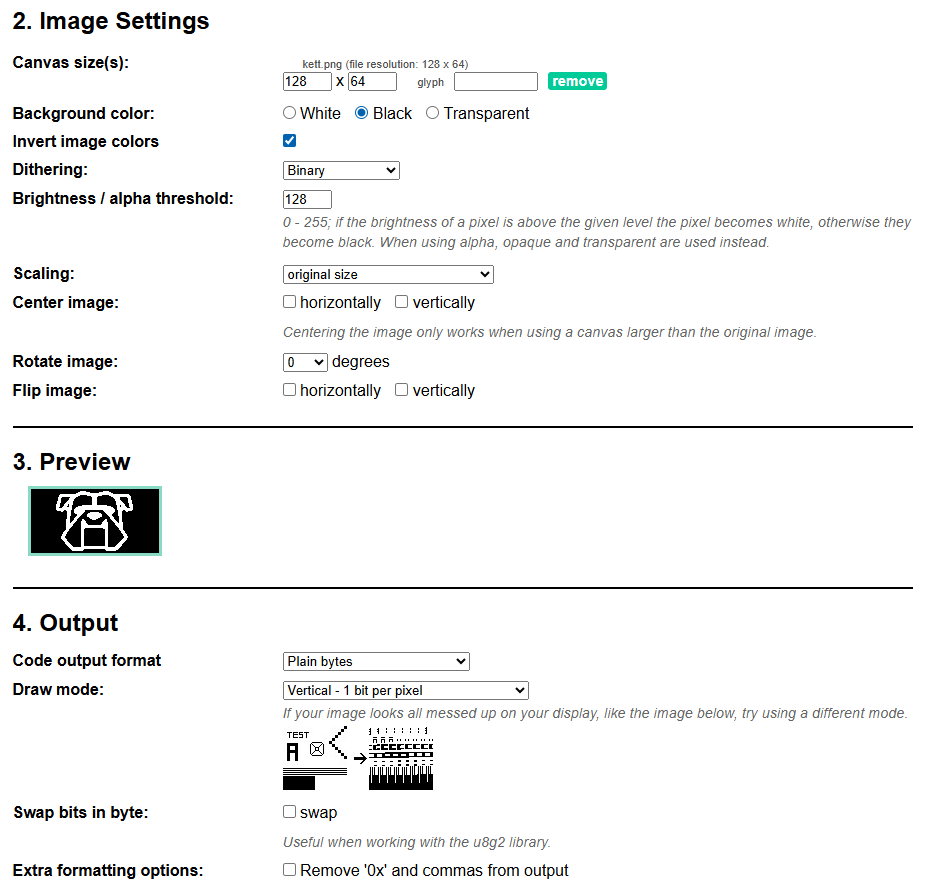
\includegraphics[width=1.00\linewidth]{figures/image2cpp-settings.png}
\captionof{figure}{image2cpp settings used to convert a 128 x 64 bitmap for the OLED screen}
\end{center}

\subsection{I2C IO Expander}

The IO expander is a Texas Instruments TCA9534 (datasheet in the datasheets folder). It adds 8 IO pins, P0 to P7, on the shared I2C bus (see I2C (software master)). Its address pins A2 to A0 are tied low on the board, which gives the address 0x20.

Each pin is an input or an output, set by the configuration register. An output is push-pull: it drives the pin high or low, and can sink up to 25 mA. The TCA9534 has no internal pull-up resistors (unlike the TCA9554): an input pin that is not connected floats and reads a random level, so an input needs an external pull-up or pull-down resistor, or a device that drives it.

The device has four registers, selected by the command byte sent after the address:
\begin{datatable}{>{\raggedright\arraybackslash}p{0.22\linewidth}>{\raggedright\arraybackslash}X>{\raggedright\arraybackslash}X}
\toprule
\textbf{Register} & \textbf{Name} & \textbf{Content} \\
\midrule
0x00 & Input port & Level on each pin, input or output (read only) \\
0x01 & Output port & Level driven on each output pin, no effect on input pins. 0xFF at power-up \\
0x02 & Polarity inversion & 1 inverts the bit of that pin in the input port register. 0x00 at power-up \\
0x03 & Configuration & 1 = input, 0 = output. 0xFF at power-up (all inputs) \\
\bottomrule
\end{datatable}

To write a register, the driver sends the address, the command byte, then the data (io\_cmd()). To read one, it sends the address and the command byte, then a repeated start, the address with the read bit, and reads the byte (io\_read\_reg()). The driver keeps a copy of the configuration and output registers in RAM, so io\_pin\_mode() and io\_write\_pin() change one bit without reading the register first. Every write updates these copies, io\_cmd() included, so the functions can be mixed. Measured on the board, io\_read() takes 0.35 ms.

\textbf{INT output: }the TCA9534 also has an open-drain interrupt output that goes low when an input pin changes, until the input port is read. The driver does not use it: read the inputs with io\_read() when they are needed.

\textbf{Note: }init\_IO\_expander() makes all the pins inputs, the safe state of the TCA9534 at power-up. Before making a pin an output, make sure nothing else drives that line: two outputs driving it to different levels can damage the pins. The output register starts at 0xFF, so a pin switched to output drives high unless io\_write() or io\_write\_pin() set it low first.
\minisec{Pins}
\begin{datatable}{>{\raggedright\arraybackslash}p{0.16\linewidth}>{\raggedright\arraybackslash}X>{\raggedright\arraybackslash}p{0.2\linewidth}}
\toprule
\textbf{Pin} & \textbf{Device} & \textbf{Direction} \\
\midrule
RC8 & I2C SDA (shared with the OLED and the accelerometer) & IN/OUT \\
RC9 & I2C SCL (shared with the OLED and the accelerometer) & OUT \\
\bottomrule
\end{datatable}
\minisec{Files}

io\_expander.c and io\_expander.h (uses i2c\_master.c and i2c\_master.h)
\minisec{Functions}
\begin{functiontable}{>{\raggedright\arraybackslash}p{0.36\linewidth}>{\raggedright\arraybackslash}X}
\toprule
\textbf{uint8\_t init\_IO\_expander(void)} & Initializes the I2C bus, makes the 8 pins inputs without polarity inversion. Returns 1 if the TCA9534 answered, 0 otherwise \\
\textbf{uint8\_t io\_read(void)} & Reads the levels of the 8 pins (input port): bit i is the level of pin Pi \\
\textbf{uint8\_t io\_read\_pin(uint8\_t pin)} & Reads the level of one pin (0 to 7): 0 or 1 \\
\textbf{void io\_pin\_mode(uint8\_t pin, uint8\_t direction)} & Makes one pin an input (IOEXP\_INPUT) or an output (IOEXP\_OUTPUT) \\
\textbf{void io\_set\_direction(uint8\_t inputs)} & Sets the direction of the 8 pins at once: bit i = 1 makes Pi an input, 0 an output \\
\textbf{void io\_write\_pin(uint8\_t pin, uint8\_t level)} & Drives an output pin high (1) or low (0) \\
\textbf{void io\_write(uint8\_t value)} & Sets the levels of the 8 output pins at once: bit i is pin Pi \\
\textbf{void io\_cmd(uint8\_t reg, uint8\_t data)} & Writes a register (IOEXP\_REG\_INPUT to IOEXP\_REG\_CONFIG in io\_expander.h) \\
\textbf{uint8\_t io\_read\_reg(uint8\_t reg)} & Reads a register \\
\bottomrule
\end{functiontable}
\minisec{Example usage}

Reading inputs and driving outputs: P0 to P3 are outputs that copy the levels of the inputs P4 to P7, and the 8 levels are shown on the OLED
\begin{lstlisting}
#include "xc.h"
#include "config.h"
#include "io_expander.h"
#include "oled.h"

void main() {
    uint8_t pins;

    init_oled();
    if (!init_IO_expander()) {
        oled_draw_string(0, "TCA9534 not found");
    }

    io_write(0x00);                // outputs low before they are enabled
    io_set_direction(0xF0);        // P4-P7 inputs, P0-P3 outputs

    while (1) {
        pins = io_read();           // bit i = level of pin Pi
        io_write(pins >> 4);        // P0-P3 copy P4-P7

        for (int i = 0; i < 8; i++) {
            oled_draw_char((7 - i) * 6, 2, (pins & (1 << i)) ? '1' : '0');
        }
        oled_update();
    }
}
\end{lstlisting}

Example 14 (``IO expander Read'' in the demo cycle) shows the levels of the 8 pins, configured as inputs, on the OLED.

\chapter{Common problems}\label{ch-common-problems}

\section{Problem 1}

When attempting to start the debugger, error

nedbg\_dspic33ck64mc105.py", line 15, in <module> from common.spitfireinterface import SpitfireException ImportError: No module named spitfireinterface

Comes up regarding a missing module in a python script used by the debugger.

\textbf{Solution}
\begin{enumerate}
\item Make sure you use the minimum required addons specified in the Curiosity Nano documentation (MPLAB X version 6.05 with device family pack ``dsPIC33CK-MC\_DFP'' version 1.6.131 and tool pack ``nEDBG\_TP'' version 1.11.554 or newer)
\item Go to Tools > Plugins
\begin{center}
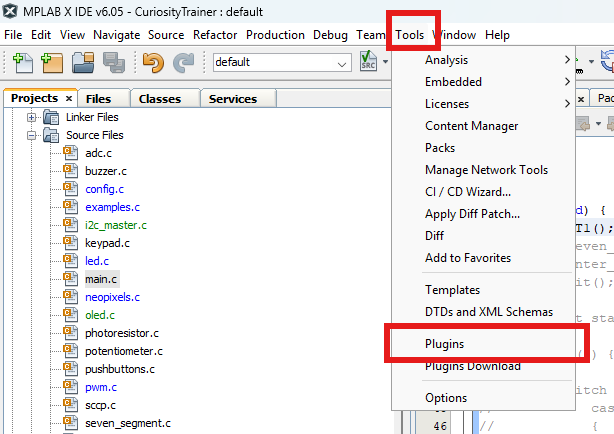
\includegraphics[width=0.98\linewidth]{figures/mplabx-plugins.png}
\captionof{figure}{MPLAB X: the Tools > Plugins window}
\end{center}
\item Check for updates, and if any, update the plugins and restart MPLAB
\begin{center}
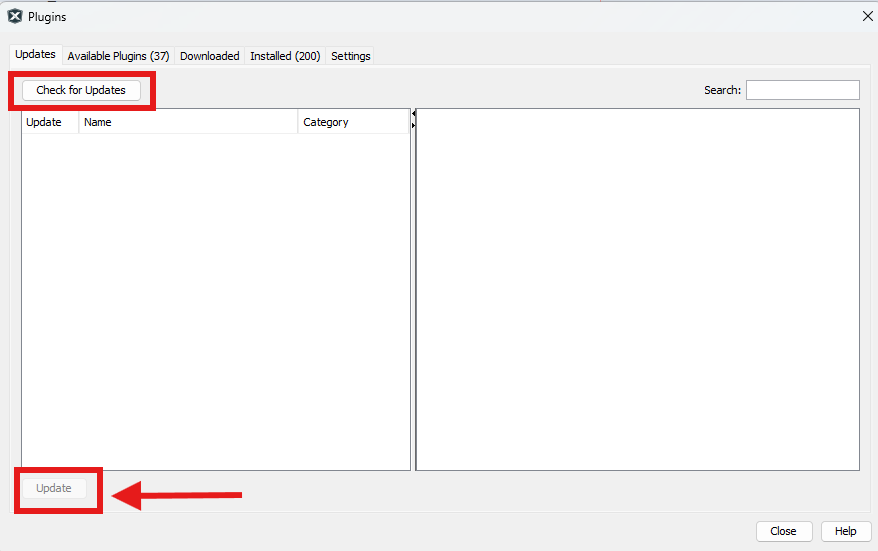
\includegraphics[width=1.00\linewidth]{figures/mplabx-plugins-update.png}
\captionof{figure}{Check for updates, then update the plugins}
\end{center}
\end{enumerate}

The error is likely caused by one of the plugins RI4; it is possible older versions of MPLAB have an outdated RI4.

\section{Problem 2}

root - ERROR - The target device is not ready for debugging. Please check your configuration bit settings and program the device before proceeding. The most common causes for this failure are oscillator and/or PGC/PGD settings.

\textbf{Solution}

In the configuration bits (in config.c), ensure that ICS is set to PGD3
\begin{center}
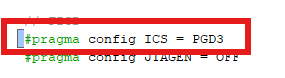
\includegraphics[width=0.46\linewidth]{figures/ics-pgd3.png}
\captionof{figure}{ICS set to PGD3 in config.c}
\end{center}

Sometimes, simply unplugging and replugging the dev board helps.

\section{Problem 3}

The serial terminal shows nothing, or only random characters, when the board sends data over UART.

\textbf{Solution}

Open the debugger's virtual COM port (for example /dev/ttyACM0 on Linux or the ``Curiosity Nano'' COM port on Windows) at 9600 8N1. On Linux, if the port was open while the board was being programmed, it may come back as /dev/ttyACM1.

Random characters mean a baud rate mismatch: FCY in config.h must match the actual clock, Fcy = 16 MHz (see Configuration).

No output at all usually means the UART pins were not mapped: PPS must be unlocked when UartInit() runs (see UART).

\section{Problem 4}

The keypad returns the wrong key, keys that are not pressed, or example 1 shows ``Keypad blocked!''.

\textbf{Solution}

Turn the slide switches SW1 to SW4 OFF: they share their pins with the keypad rows (see Keypad). In your own code, call keypad\_check\_rows() before readKey() and ignore the keypad while it returns a non-zero value.

\section{Problem 5}

The build fails with ``Link Error: Could not allocate section .ndata'' (or .nbss).

\textbf{Solution}

The 4 KB of near data memory is full. Declare large arrays (buffers of hundreds of bytes) static with \_\_attribute\_\_((far)), and never define variables in a header file: a definition in a header, such as static uint8\_t fb[1024] that used to be in oled.h, creates a separate copy in every file that includes it.

\end{document}
